\newpage
\section{Classification of Self-Adaptive Systems}
\label{ch:SASClassification}

% TODO: maybe provide a fictional example to explain SAS
% - useful for understandability
%   - Which parts can not be optimized: why the environment generally can not be controlled.

% TODO:
% - Shortly cover how SAS are classified:
%     - Krupitzer et al
%     - "Towards a taxonomy ..."
% - Which parts can be optimized?
% - Which parts cant be optimized/are a design decision?
% - Current landscape of OA
%     - mostly ML

% \begin{itemize}
%     \item How Self-Adaptive Systems are classified.
%     \item Which parts of Self-Adaptive Systems can be optimized or are important for optimization.
%     \item An overview of current optimization approaches for Self-Adaptive Systems.
% \end{itemize}

% \paragraph*{Literature for this section:} \begin{itemize}
%     \item "A survey on engineering approaches for self-adaptive systems" \cite{SurveyOnEngineeringApproaches}
%     \item "Towards a Taxonomy for the Evaluation of Self-* Software" \cite{TaxonomyOfSelfSoftware}
%     \item "Dissecting Self-* Properties" \cite{DissectingSelfProperties}
%     \item "Self-Adaptive Software: Landscape and Research Challenges" \cite{LandscapeAndResearchChallenges}
%     \item "The Application of Machine Learning in Self-Adaptive Systems: A Systematic Literature Review" \cite{ApplicationOfMachineLearning}
%     \item "Comparison of Approaches for Self-Improvement in Self-Adaptive Systems" \cite{ComparisonOfSelfImprovement}
% \end{itemize}

% TODO: How are SAS classified
There are different approaches on how to classify and describe Self-Adaptive Systems,
which all focus on different usages, the three approaches that will be highlighted by this paper are:
% TODO: Add usages
\begin{itemize}
    \item FORMS from Weyns et al., 2012 \cite*{FORMS}
    \item Raibulet's, 2018 taxonomy for self-* properties \cite*{TaxonomyOfSelfSoftware}
    \item Krupitzer's et al., 2015 taxonomy for Self-Adaptive Systems \cite*{SurveyOnEngineeringApproaches}
\end{itemize} 

%% FORMS
% - reflection
\par
In their 2012 paper FORMS \cite{FORMS} Weyns et al. propose a formal reference model for describing Self-Adaptive Systems.
By composing a Self-Adaptive System from different levels of components called subsystems,
where each level can adapt the level beneath, FORMS models the self-adaptive process using reflection.
The bottom level is populated by base-level computations, base-level subsystems and domain models.
On top of these base-level components are reflective computations, reflective subsystems and reflection models.

The goal of FORMS is to provide a well defined basis for talking and reasoning about Self-Adaptive Systems.
This is achieved by providing a definition of FORMS, which classifies Self-Adaptive Systems, using Z notation.

%% self-* properties
% - read the paper

%% Krupitzer
\begin{figure*}[hbt!]
    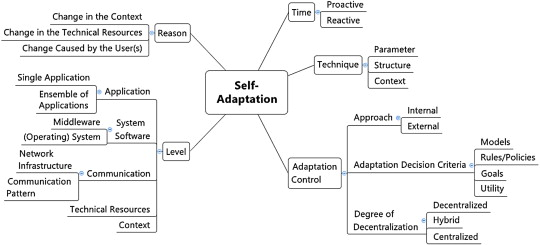
\includegraphics[width=\textwidth]{images/KrupitzerTaxonomy.jpg}
    \caption{Taxonomy for \acrlong{sas} by Krupitzer et al., 2015 \cite*{SurveyOnEngineeringApproaches}}
    \label{fig:KrupitzerTaxonomy}
\end{figure*}

\par
The taxonomy for Self-Adaptive Systems by Krupitzer's et al., 2015 \cite*{SurveyOnEngineeringApproaches} in Figure \ref{fig:KrupitzerTaxonomy}
is based upon the 5W+1H questions by Salehie and Tahvildari, 2009 \cite*{LandscapeAndResearchChallenges}.
These questions are: Where, When, What, Why, Who and How.
Each of these questions is responsible for a different aspect of Self-Adaptive Systems and corresponds to a dimension of the taxonomy. \\

% Why
First there needs to be a reason for a Self-Adaptive System to adapt.
Why an adaptation should be performed is answered by the Reason dimension.
According to the taxonomy reasons for an adaptation can be changes in either the context, a technical resource or changes caused by the user. \\

% Where
The question of where asks on which level of the system changes need to occur.
The different levels on which changes can occur include:
\begin{itemize}
    \item Different levels of applications from the operating system to a user application.
    \item How systems communicate with each other.
    \item The technical resources that are needed by the system.
    \item The context in which the system operates.
\end{itemize}

% When
While the original When-Question by Salehie and Tahvildari tries to understand all temporal aspects of Self-Adaptive Systems,
including how frequently changes should occur and if they happen continously,
the taxonomy only answers the question when changes should be performed.
For this purpose the Time dimension differentiates between systems that perform changes proactively or reactively. \\

% What
In addition to the question of where and when changes should occur, it is also important to know
what changes should occur. There are different techniques, that can be used.
The Technique dimension of the taxonomy differentiates between systems that change parameters, their structure or their context. \\

% Who
After answering where, when, what and why changes should be performed, 
it is necessary to select who is responsible for these changes.
According to Salehie and Tahvildari it is also important to establish if the changes can be performed fully autonomous
or if the involvement of human operators is necessary.
The taxonomy does not directly address all of these concerns but states that:
"N/A (nature of a SAS leads to an automatic type of adaptation)" (Krupitzer et al., 2015 \cite{SurveyOnEngineeringApproaches}). \\

% How
Lastly, after determining the where, when, what, why and by who, there needs to be a way
to perform the required changes. This is answered by asking how the changes should be performed
and corresponds to the Adaptation Control.
The three main factors of the Adaptation Control are the degree of decentralization, the adaptation decision criteria
and the approach taken by the system, which divides Self-Adaptive Systems into those where the adaptation logic is part of the application logic
and those with separated adaptation and application logic.

% TODO: Which parts cant be optimized/are a design descision
% - the environment / reason for a change
% - time: mostly a design decision
% - level: 
% - who: in THE taxonomy not included

After classifying Self-Adaptive Systems.
The following question can be asked: Which parts of a Self-Adaptive System can be optimized?
To answer this we will start by looking at which parts can not be optimized. % TODO: seems harsh: or seem like design

The first part that can not be optimized is the environment which provides the Reason dimension.
While the environment for a Self-Adaptive System can be choosen in a way which is most beneficial for the system
and can be influenced by actors, % TODO: stand in einem Paper, wahrscheinlich FORMS
the behaviour of the systems environment can generally not be controlled completly.

Another dimension of Self-Adaptive Systems that can not be optimized, or is not useful to optimize,
is the Time dimension. This dimension is mostly design decision on how the system should behave and be constructed.
It is also a question of how to handle uncertainty and the level of accepted risk.
A proactive system can prevent faults and degredation in Quality-of-Service metrics 
but it can also predict the wrong changes, which can lead to a situation where the system itself generates faults by
reacting in a way that is different or opposite to the currently needed change. % TODO: besser formulieren
A reactive system can not prevent faults like a proactive system
but its behavior can be much more stable because it only has to react to a change and not also predict that change.

% TODO: ???
The Level dimension is mostly a design decision?

Lastly the question of who is responsible can not be optimized because it is trivially answered b

% TODO: Which parts can be optimized
% - Adaptation control
% - Technique

The two remaining dimensions can be optimized. These are the Adaptation Control and the Technique.

The Approach and the Degree of Decentralization used by the Adaptation Control can not be optimized 
because they are design decisions of how the system is built.
But the Adaptation Decision Criteria can be optimized. An optimization of the Adaptation Decision Criteria
could for example be to dynamically adapt the rules and policies at runtime to better reflect a changing environment.

Another dimension that can be optimized is the Technique. 
This can be optimized by changing what gets adapted by the system.

% TODO: Current landscape